\documentclass[12pt,titlepage]{article}

% \usepackages21{fancyhdr}

\usepackage[printwatermark]{xwatermark}

\usepackage{grffile}
\usepackage{xcolor}
\usepackage{lipsum}
\usepackage{times}
\usepackage{soul}
\usepackage{epsfig}
\usepackage{rotating}
\usepackage{url}
\usepackage{latexsym}
\usepackage{graphicx}
\usepackage{amsfonts}
\usepackage{amsmath, amsthm, amssymb}
\usepackage{fullpage}
\usepackage{setspace}
\usepackage{natbib}
\usepackage{longtable}
\usepackage{keyval}
\usepackage{caption,subcaption}
\usepackage{arydshln}
%%\usepackage[hyphenbreaks]{breakurl}

%% allow urls to get broken on hyphens
\usepackage{hyperref}
\def\UrlBreaks{\do\/\do-}


%% APSR submission: no commas in citations between name and year
%% See http://merkel.zoneo.net/Latex/natbib.php
\bibpunct{(}{)}{;}{author-year}{}{;}

% the opening bracket symbol, default = (
% the closing bracket symbol, default = )
% the punctuation between multiple citations, default = ;
% the letter `n' for numerical style, or `s' for numerical superscript style, any other letter for author-year, default = author-year;
% the punctuation that comes between the author names and the year
% the punctuation that comes between years or numbers when common author lists are suppressed (default = ,);

\usepackage{footmisc}
\renewcommand{\footnotelayout}{\doublespacing} % set spacing in footnotes
\newlength{\myfootnotesep}
\setlength{\myfootnotesep}{\baselineskip}
\addtolength{\myfootnotesep}{-\footnotesep}
\setlength{\footnotesep}{\myfootnotesep} % set spacing between footnotes

% make footnote font size same as regular font size in text
\renewcommand{\footnotesize}{\normalsize} 


%% Use this for a "DRAFT" watermark
%% \newwatermark[allpages,color=pink!50,angle=45,scale=5,xpos=-25,ypos=40]{DRAFT}

%% List all locations for graphics here
\graphicspath{ {../plots/} }


\begin{document}
\sloppy
\thispagestyle{empty}

%% APSR submission requires double-spaced footnotes
%%\newcommand{\footnote}[1]{\footnote{\doublespacing #1}} %% <-- note \doublespacing here.

\renewcommand{\topfraction}{.85}
\renewcommand{\bottomfraction}{.7}
\renewcommand{\textfraction}{.15}
\renewcommand{\floatpagefraction}{.66}
\renewcommand{\dbltopfraction}{.66}
\renewcommand{\dblfloatpagefraction}{.66}

\newcommand{\Yi}{\ensuremath{Y_i}}

% \urldef\myurlncsl1\url{foo%.com}
% \begin{document}
% text\footnote{WWW: \myurl}


\title{\Large{All in the family:\\German twin finishing times in\\the
    2016 women's Olympic marathon}}\author{David
  Cottrell\thanks{Postdoctoral Research Fellow, Program in
    Quantitative Social Science, Dartmouth College, 6108 Silsby Hall,
    Hanover, NH 03755 (\texttt{david.cottrell@dartmouth.edu}).} \and
  Michael C.\ Herron\thanks{Visiting Scholar, Hertie School of
    Governance, Berlin, Germany, and Professor of Government,
    Dartmouth College, 6108 Silsby Hall, Hanover, NH 03755
    (\texttt{michael.c.herron@dartmouth.edu}).}}


\maketitle \doublespacing 

%\begin{abstract} 
% \noindent
%The abstract
%\end{abstract}

%\newpage


\begin{quote}
  \emph{``I invested all I had and 300 meters before the finish line,
    I was next to Lisa. It was a magical moment that we could finish
    this marathon together. We did not think about what we were
    doing.'' -- Anna Hahner}
\end{quote}


\section*{Introduction}

At 9:30am on August 14, 2016, the women's Olympic marathon kicked off
in Rio de Janeiro, Brazil, when 156 runners from 80 countries across
the world left the starting line en route to their destination 42.195
kilometers away. Two hours, twenty-four minutes, and four seconds
later, Jemima Sumgong of Kenya would be the first to cross the
finishline and take home gold; Sumgong was just three and one-half
minutes slower than her prior personal best time in the
marathon. Approximately 21 minutes later, twin marathoners from
Germany, Anna and Lisa Hahner, would cross the finishline together,
holding hands and celebrating a personal victory. Although the Hahners
would finish 81st and 82nd, respectively, well behind the winners of
the marathon, Anna Hahner would describe their joint finish as a
``magical moment.''


%% Honigkuchenpferde reference
%%
%% https://www.welt.de/sport/olympia/article157669264/Das-falsche-Laecheln-der-deutschen-Lauf-Zwillinge.html 

The media quickly picked up the Hanher story as an image of the
beaming twins, finishing hand-in-hand, captured a public
audience. While many believed the twin's near-simultaneous finish was
a reflection of Olympic spirit, not everyone agreed with this rosy
interpretation. The twins' happy facial expressions at the finish were
portrayed as a bit contrived---smiling like ``Honigkuchenpferde,''
cookies in the shape of a horse, was the description offered by one
editorialist---and the sports director of the German Athletics
Federation, Thomas Kurschilgen, stirred up controversy when he
suggested that the Hahners' photo-finish was no coincidence.
Kurschilgen averred that the twins slowed down so as to finish
simultaneously and create a spectacle, and he justified his charge by
noting that the Hahners ran the Rio marathon over 18 minutes slower their
personal best times prior to the Olympics.  Kurschilgen's accusations
were denied by the Hahner twins, perhaps not surprisingly, who claimed
that their joint finish was simply a fortuitous coincidence.

%% Honigkuchenpferd quote from here:
%%
%% https://www.welt.de/sport/olympia/article157669264/Das-falsche-Laecheln-der-deutschen-Lauf-Zwillinge.html

What happened in the women's Olympic marathon in Rio, and how might we
develop a statistical approach that assesses whether the Hahner twin's
finish in the race was coincidental or intentional?  These two
interpretations are clearly at odds. If the former, then the Hahners
are to be celebrated and their finish treated as an expression of the
spirit behind the Olympic games. If the latter, though, then the twins
may have violated this spirt by not trying hard enough. It is perhaps
too easy for us to write such a glib sentence---neither of us can
fathom being able to complete a marathon anywhere in the vicinity of
two and a half hours---but we nonetheless want to know what the data
from the Olympic marathon tell us.

%% Was the Hahner finish in the 2016 women's Olympic marathon a lovely coincidence or something else?

Among female Olympic marathoners, the Hahner twins were not alone in
sharing familial ties.  The Rio marathon also featured twins from
North Korea, Kim Hye-song and Kim Hye-gyong, who posted identical
times and finished 10th and 11th in the race, respectively. The Kim
finish, unlike the Hahner finish, appears devoid of post-race
controversy. Moreover, three triplets from Estonia competed in the Rio
marathon, although only two, Lily Luik and Leila Luik, finished it, in
97th and 114th place, respectively. The third Estonia triplet, Liina
Luik, recorded what is known as a DNF---an abbreviation that means did
not finish.  Although our focus here is the Hahner twins, we touch on
the Kim twins and Luik triplets in the course of what follows.

\section*{Marathon data and our research design}

For each participant who started the women's Olympic marathon, we know
several things: personal best marathon time prior to the 2016 Olympic
games; age; split times from the Rio marathon course at 5 kilometers,
10 kilometers, and so forth; and, overall finishing time. We cannot
directly observe the effort that an individual put into the race, and
we do not know why some runners have DNF results.  Some runners may
have injured themselves on the course and accordingly dropped out, and
others may have stopped running, uninjured, in anticipation of an
unsatisfactory result. Of 156 marathon starters, 133 completed the
race and 23 DNFed at various locations throughout the course. The
overall DNF rate was thus $\frac{23}{156} \approx 0.15$, and the
relatively small sample size at our disposal yields a relatively wide
95\% confidence for this rate, namely, $\left(0.098, 0.22\right)$.

Kurschilgen's accusation against the Hahner twins has two components,
that these two women ran slowly \emph{and} that they finished
simultaneously.  We suspect that Kurschilgen would not have expressed
ire at the Hahners had they finished in 1st and 2nd place in Rio,
hand-in-hand with wide grins.  Thus, our investigation of the charges
that Kurschilgen offered distinguishes between a slow finish and a
simultaneous finish.

Our research design is twofold.  First, we present visualizations that
describe various features of the 2016 women's Olympic marathon, and
among other things our visualizations feature difference between
runners' Rio times and their prior personal best marathon times.  The
visualizations suggest that the Hahner twin's pace in the marathon was
slow, albeit not excessively so, but that their simultaneous finish
was quite unusual given the twins' differences in abilities (and
similarly for the Kim twins).  We then turn to a regression-based
simulation of the marathon, and our simulations reinforce what we
observed in prior visualizations, namely, that the Hahner twins did
not run appreciably slowly yet finished suspiciously close to each
other.  We return in our conclusion to Kurschilgen's claims about the
Hahners and offer thoughts about their validity.

\section*{Visualizing the Olympic marathon}

One way that we might assess whether a women marathoner's Rio finish
was unusual---or, say, whether two finishes were jointly unusual---is
by comparing a runner's observed Olympic finishing time on August 14,
2016, with a measure of her underlying marathon talent.  For the
latter we use prior personal best marathon times.  This is a natural
measure of marathon talent, we believe, but it is not entirely free of
complications.  For example, personal best times are potentially
confounded by the marathon courses on which they were set; some
courses, like the Berlin marathon, are known for relatively fast
times.  In addition, personal best times may be confounded by
conditions, like weather, that varied across races.  Finally, personal
best times may not capture Olympic raceday idiosyncrasies that could
affect individual runners.  For example, a runner could have woken up
with a minor cold on the morning of August 14, 2016.  With these
concerns in mind, we use a runner's half marathon split time from the
Olympic marathon as a secondary measure of athletic skill in
marathoning.  

Figure \ref{fig:scatter} contains two plots describing how finishing
times from the Rio women's marathon varied as a function of athletes'
personal best times and half marathon split times.  The points in the
plots are colored by twin/triplet status, and both plots
contain %second-order polynomial regression lines.
dashed lines representing least squares regression fits.  The ticks
along the horizontal axes in both plots indicate times, either
personal bests or half marathon splits, of runners who earned DNF
results.\label{scatterplots}

\begin{figure}[!ht]
  \centering
  \caption{Olympic finishing times as a function of underlying marathon talent}
  \label{fig:scatter}
  \begin{subfigure}{.495\textwidth}
    \centering
    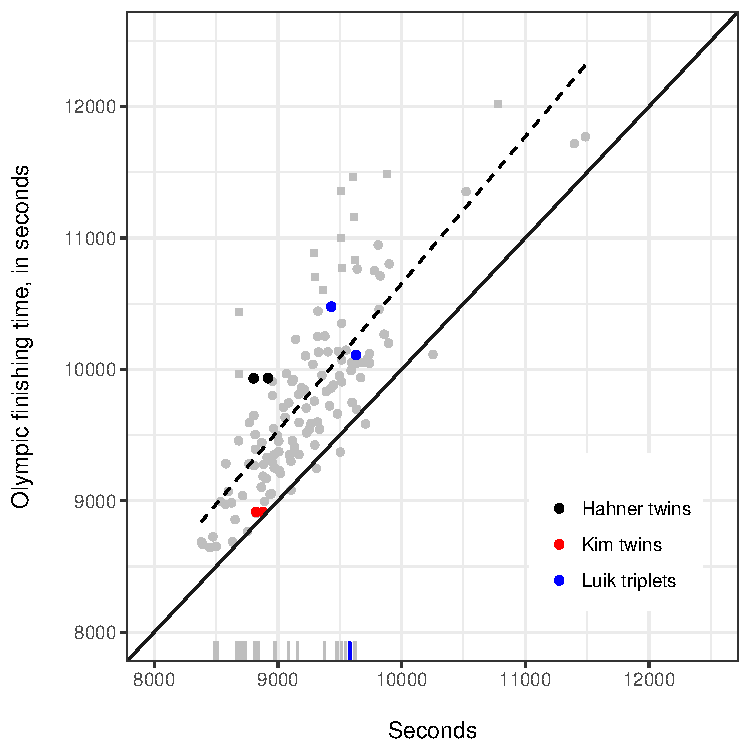
\includegraphics[width=\textwidth, keepaspectratio]{scatter_plot_no_quadratic.pdf}
    \caption{Based on personal best} 
    \label{fig:45degreeplot}
  \end{subfigure}
  \begin{subfigure}{.495\textwidth}
    \centering
    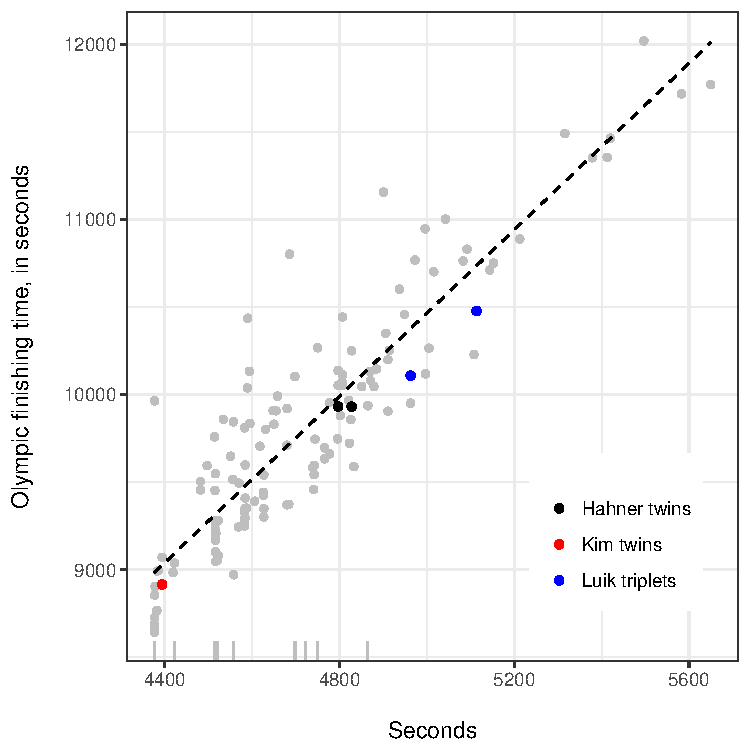
\includegraphics[width=\textwidth, keepaspectratio]{scatter_plot_half_no_quadratic.pdf}
    \caption{Based on half marathon split} 
    \label{fig:45degreeplot_half}
  \end{subfigure}
\end{figure}

Considering first the relationship between Olympic finishing and
personal best times, Figure \ref{fig:45degreeplot}'s solid 45-degree
line is informative.  Given the paucity of points (only five of them)
below this line, it follows that the vast majority of Olympic
marathoners ran slower in Rio compared to their prior personal bests.
The Hahner twins were definitely on the slow side, well above the
45-degree line, but a number of runners had even greater differences
between their Olympic times and their personal bests than the Hahners.
These runners are denoted with squares in Figure
\ref{fig:45degreeplot}, and there are 13 such symbols, highlighting
approximately 10\% of the racers who completed the Rio marathon.
Moreover, the figure shows that there were two women who had personal
best times slightly faster than the Hahners and yet finished after the
two German women.  Although Figure \ref{fig:45degreeplot} suggests
that the Hahner twins were slower than one would have expected given
their previous best marathon times, it is not consistent with the
accusation that they dramatically slowed down in the Rio marathon.

% > df <- read.csv("data/times.csv", stringsAsFactors = FALSE) %>% tbl_df()
% > df <- df[df$BIB != 1172,]
% > sort(dta$FINAL - dta$PB) / 60
%   [1] -2.3333333 -2.2166667 -2.0666667 -1.1166667 -0.4000000  0.2166667
%   [7]  0.6333333  0.9000000  1.0166667  1.3666667  1.5166667  1.7166667
%  [13]  1.7666667  1.8500000  2.1166667  2.4666667  2.5333333  3.0166667
%  [19]  3.0500000  3.1666667  3.2666667  3.2833333  3.3666667  3.4500000
%  [25]  3.6833333  3.9000000  3.9833333  4.2000000  4.2666667  4.3833333
%  [31]  4.4666667  4.5833333  4.6166667  4.6333333  4.6833333  4.7333333
%  [37]  4.7333333  4.8333333  5.0666667  5.0833333  5.0833333  5.1000000
%  [43]  5.1333333  5.3500000  5.3500000  5.4000000  5.7166667  5.7333333
%  [49]  5.9333333  6.0000000  6.0333333  6.1166667  6.3333333  6.3500000
%  [55]  6.5000000  6.5333333  6.6000000  6.6666667  6.7166667  6.7833333
%  [61]  6.8166667  6.9500000  7.1000000  7.1500000  7.2000000  7.3500000
%  [67]  7.4500000  7.5666667  7.6000000  7.6000000  7.6333333  7.7500000
%  [73]  7.8833333  7.9666667  7.9833333  8.3000000  8.6000000  9.3000000
%  [79]  9.5500000  9.5833333  9.6000000  9.7166667  9.9500000  9.9833333
%  [85] 10.3166667 10.5333333 10.6666667 10.7000000 10.8333333 10.9666667
%  [91] 11.1500000 11.1833333 11.4666667 11.7166667 12.1666667 12.6000000
%  [97] 12.9166667 13.2166667 13.2833333 13.3833333 13.7666667 13.8666667
% [103] 13.9166667 14.0500000 14.0833333 14.5666667 14.6833333 14.7500000
% [109] 15.0000000 15.0500000 15.5000000 15.9000000 16.2000000 16.9000000
% [115] 17.4500000 18.1000000 18.6666667 18.7166667 18.8000000 18.9333333
% [121] 20.1500000 20.6333333 20.7000000 20.8500000 21.3500000 23.4166667
% [127] 24.9333333 25.6500000 26.5666667 26.7666667 29.2166667 30.7000000
% [133] 30.9666667
% > 

With respect to our second measure of marathon skill, Figure
\ref{fig:45degreeplot_half} shows that there was nothing abnormal
about the Hahner twins' overall finishing times, conditional on their
half marathon splits. As one might expect, a runner's time halfway
through the course is a fairly strong predictor of her finishing time.
Here we see that the relationship between the Hahner twin's half
marathon split times and their finishing times is similar to that of
other Rio runners.  The two points representing the Hahners are in the
middle of the distribution of points and therefore imply that the
twins do not seem to have slowed down dramatically after their reached
the halfway point of the Rio marathon.  This is consistent with the
aforementioned Figure \ref{fig:45degreeplot} and inconsistent with
accusations made against the Hahner twins, at least the part of the
accusation that focused on their overall pace.

Another perspective on the extent to which the Hahners' overall
marathon finishing times were not unusual can be gleaned from Figure
\ref{fig:residuals}.  This figure presents cumulative distributions of
the residuals from the regression models displayed in the two panels
of Figure \ref{fig:scatter}.  In particular, we calculated the
residuals from Figures \ref{fig:45degreeplot} and
\ref{fig:45degreeplot_half}, Studentized them, and then arranged
resulting Studentized residuals from least to most along the
horizontal axes in Figures \ref{fig:studentizedresiduals} and
\ref{fig:studentizedresiduals_half}.\label{residualplots}

\begin{figure}[!ht]
  \centering
  \caption{Studentized residuals from Olympic finishing time regressions}
  \label{fig:residuals}
  \begin{subfigure}{.495\textwidth}
    \centering
    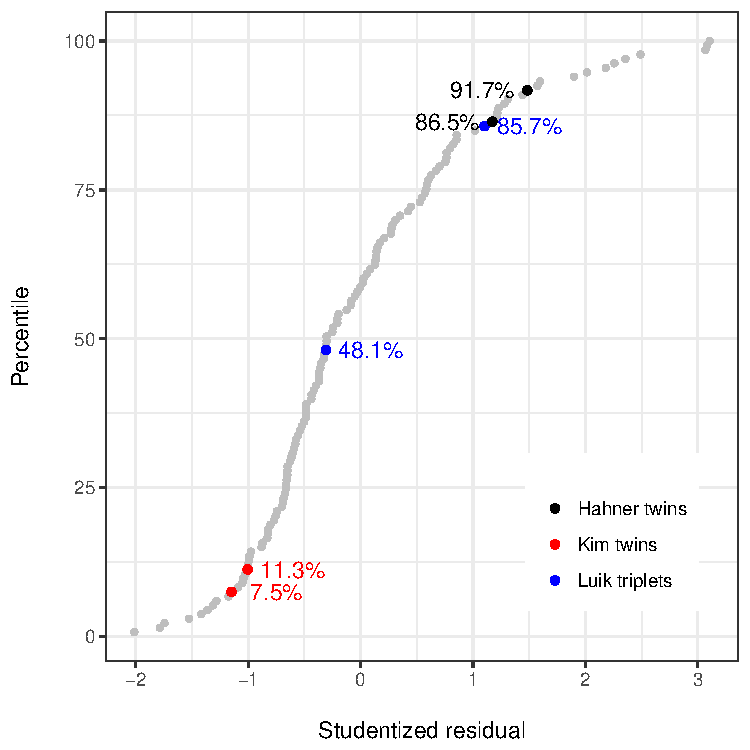
\includegraphics[width=\textwidth, keepaspectratio]{studentized_residuals_no_quadratic.pdf}
    \caption{Based on personal best} 
    \label{fig:studentizedresiduals}
  \end{subfigure}
  \begin{subfigure}{.495\textwidth}
    \centering
    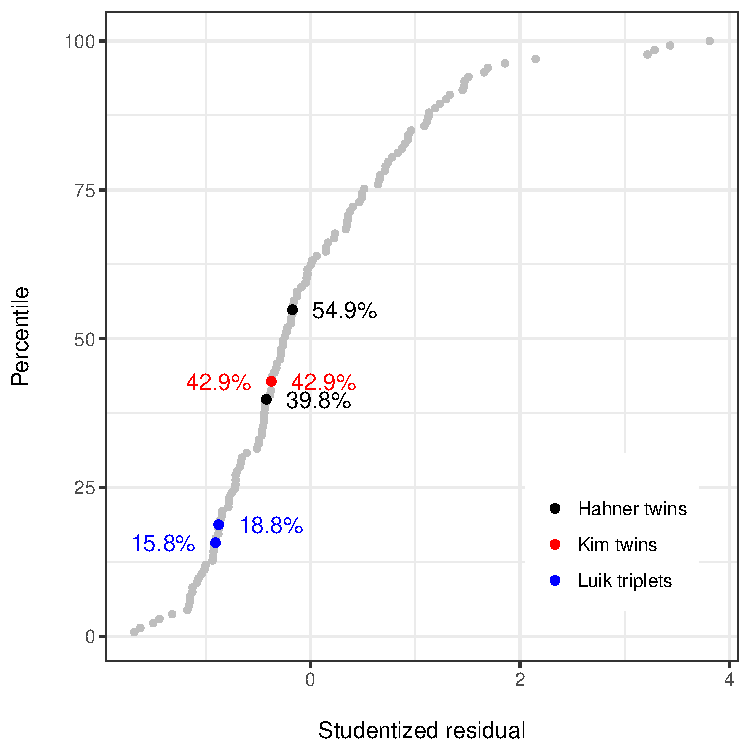
\includegraphics[width=\textwidth, keepaspectratio]{studentized_residuals_half_no_quadratic.pdf}
    \caption{Based on half marathon split}
    \label{fig:studentizedresiduals_half}
  \end{subfigure}
\end{figure}

The cumulative residuals depicted in the two panels of Figure
\ref{fig:residuals} are consistent with our interpretation of the
Hahner twin's Olympic finishing times as not particularly
remarkable. With personal best time as a measure of marathon talent as
in Figure \ref{fig:studentizedresiduals}, the two Hahner residuals are
in the right tail of the residual distribution; however, their
locations are not extreme.  One residual is located at the 87th
percentile and the other at the 92nd.  While these two residuals are
in the tail end of the residual distribution, they are not major
outliers that would lead us to think that the Hahner twin's marathon
finishing times were extremely slow.  Moreover, the residuals for the
Kim twins are similarly not remarkable; these two residuals are in the
left tail of the residual distribution, indicating that the Kims ran
faster than one would have expected.  Finally, if one relies on half
marathon split times as measures of marathon talent, as in Figure
\ref{fig:studentizedresiduals_half}, similar conclusions follows.
Neither Hahner twin had a finishing time that was particularly unusual
given her half marathon split, and this applies to the Kim twins as
well.

If the Hahner twins did not slow down excessively, might they have run
somewhat strategically at the end of the Olympic marathon in order to
generate a simultaneous finish?  We now offer a visualization that
speaks to this question.

The personal best times of the Hahner twins were 115 seconds apart and
their official finishing times were separated by one second.  Is such
a 115 to one compression typical among pairs of runners?  Relatedly,
are there other pairs of Olympic marathoners who had a difference
between personal best times of 115 seconds apart and, if so, how close
were their finishing times?

Of the 133 marathon finishers, there are $\binom{133}{2} = 8,778$
pairs of runners.  Of these and ignoring the Hahner twins, ten had
exactly a 115 second gap in personal best times.  Differences in
finishing times of these ten pairs, in seconds, are as follows: 36,
93, 172, 319, 379, 459, 552, 671, 675, and 739.  In other words, of
all pairs of runners in the Rio marathon who had a personal best
difference that was equivalent to the Hahner twins' difference, the
twins had the greatest compression based on finishing time.

% df2b[abs(df2b$pb_diff)==115,]
% # A tibble: 11 × 8
%                       name_i              name_j pb_diff result_diff
%                        <chr>               <chr>   <int>       <int>
% 1                Anna Hahner         Lisa Hahner    -115          -1
% 2                  Lily Luik Mariya Korobitskaya     115          36
% 3        Lisa Jane Weightman      Lanni Marchant    -115          93
% 4           Irina Smolnikova      Viviana Chávez     115        -172
% 5              Sonia Samuels    Helalia Johannes     115        -319
% 6  Jessica Draskau-Petersson       Gladys Tejeda     115         379
% 7        Maryna Damantsevich       Gladys Tejeda     115         459
% 8          Panayióta Vlaháki     Matea Matosevic    -115         552
% 9         Nataliya Lehonkova       Olha Kotovska     115         671
% 10               Anja Scherl      Desireé Linden     115         675
% 11              Rose Chelimo    Helalia Johannes    -115        -739
% # ... with 4 more variables: diff_in_diff <int>, consecutive <lgl>,
% #   twins <chr>, PERCENTILE <dbl>
% > 

\begin{figure}[!ht]
 \caption{Pair-wise differences in Olympic finishing times and
   differences in marathon talent}
  \label{fig:diffdiff}
 \centering
 \begin{subfigure}{.49\textwidth}
 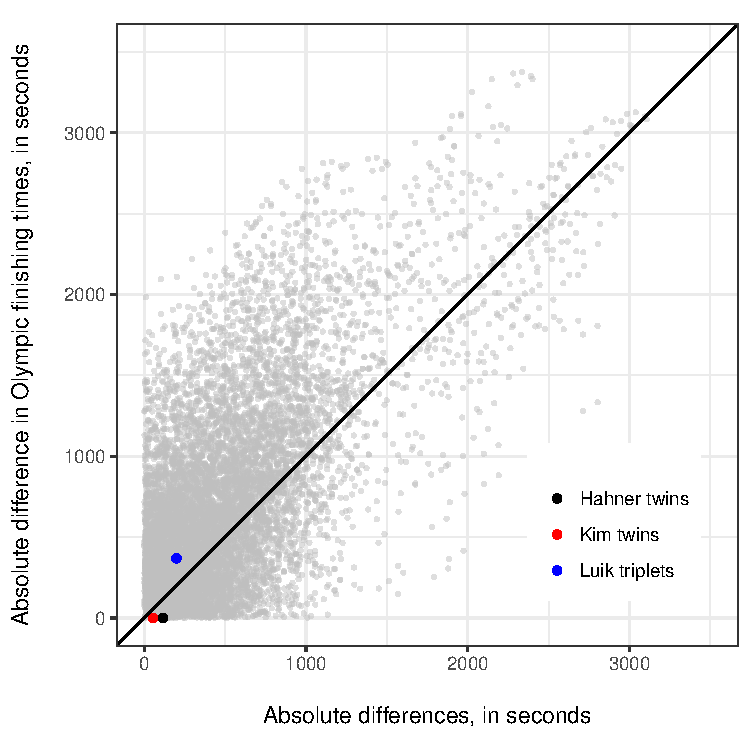
\includegraphics[width=\textwidth, keepaspectratio]{diff_in_diff_scatter_plot.pdf}
 \caption{Based on differences in personal best times}
  \label{fig:diffdiffscatter}
 \end{subfigure}
  \begin{subfigure}{.49\textwidth}
 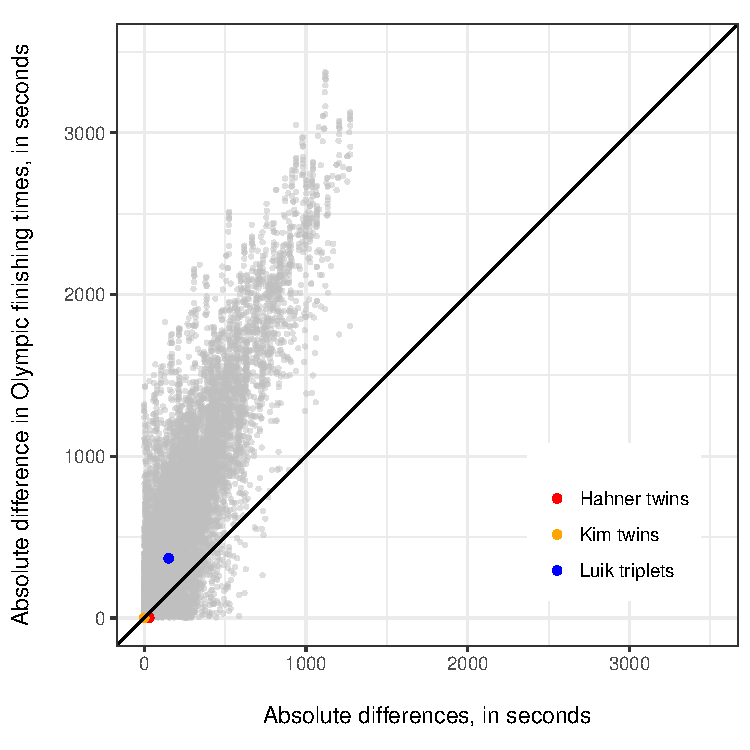
\includegraphics[width=\textwidth, keepaspectratio]{diff_in_diff_scatter_plot_half.pdf}
 \caption{Based on differences in half marathon splits}
  \label{fig:diffdiffscatterhalf}
 \end{subfigure}
\end{figure}

We can generalize this result by looking at all pairs of runners in
the marathon.  For all 8,778 pairs of 133 finishers, Figure
\ref{fig:diffdiffscatter} plots differences in finishing times against
differences in personal best times, and pairs of twins/triplets are
identified by the same color scheme we used earlier (recall that only
two of the Luik triplets finished the Rio marathon).  Consider first
the Hahner twins.  The two German women are effectively located on the
horizontal axis because their difference in finishing times is one
second.  However, there are many points above the Hahners' black dot,
and this shows that, conditional on an approximate 115 second
difference in personal best times, most marathoner pairs did not have
close finishing times like the Hahners.  Some pairs of runners with
around 115 second personal best differences had finishing time
differences of 1,000 seconds, i.e., in excess of 15 minutes.  The
points in Figure \ref{fig:diffdiffscatter} are not independent, but
they provide a rough sense of the dispersion in finishing time
differences between runners that one might expect conditional on
differences in personal best times.

Thinking about the accusations leveled against the Hahner twins,
Figure \ref{fig:diffdiffscatter} suggests that Anna and Lisa Hahner
did indeed run with an eye on each other.  In fact, the same can be
said of the Kim twins, who ran seemingly in lockstep throughout the
entire Rio marathon.  The North Korean twins had a personal best
difference of 53 seconds and a finishing time difference of literally
zero seconds.  Beyond these twins, there were eight pairs of Rio
runners with a 53 second personal best difference, and resulting
finishing time differences are as follows: 9, 51, 228, 340, 352, 571,
662, and 751.  As in the Hahner case, the Kim twins compressed their
finishing times---meaning that they finished with less time between
them than the difference in their personal bests---more than any other
pair of runners with similar personal best differences.

Similar conclusions follow from Figure \ref{fig:diffdiffscatterhalf},
which plots pair-wise differences between Olympic finishing times and
half marathon split times.  Namely, many pairs of runners had similar
differences in half marathon times as the Hahner and Kim twins, but
the vast majority of these pairs did not have close finishing times.

Figure \ref{fig:secondsbehind} describes each Olympic runner's status
at various split times on the marathon course.  Each dot in the
figure---colored as before---depicts a recorded split and the number of
seconds each runner was behind the race leader at the time.  There are
more dots at earlier splits due to subsequent DNFs. 

\begin{figure}[!ht]
  \centering
  \caption{Runner status by split}
  \label{fig:secondsbehind}
  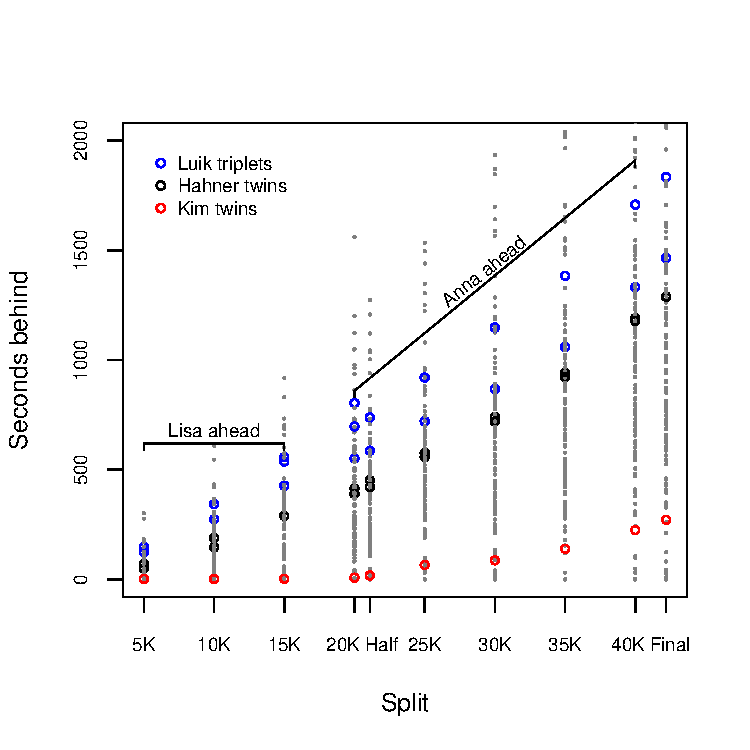
\includegraphics[scale = 1]{seconds-behind.pdf}
  % \begin{flushleft}
  %   \emph{Note: each dot represents one runner at a split.  DNFs are
  %     not pictured, and splits are not to scale.}
  % \end{flushleft}
\end{figure}

The Estonian triplet DNF prior to the half marathon split is evident
in Figure \ref{fig:secondsbehind} , which also shows that Lisa Hahner
was ahead of her sister through 15 kilometers.  The figure contains
two red dots representing the North Korean Kim twins, but this is not
visually apparent because the Kim twins had identical split times
during the entire marathon.  This explains why we used the term
``lockstep'' to refer to the Kim twin's marathon pace.

\section*{Simulating the Marathon}

% The Hahner sisters claimed that they ran the marathon independent of
% each other.  Their simultaneous finish was no more than a product of
% ability and luck.  One might expect such a finish given that their
% personal best marathons are within 114 seconds of each other.  Add a
% little bit of luck to the occasion and, as the twins have claimed all
% along, one might easily argue that the simultaneous finish is simply a
% joyous coincidence rather than a wholly implausible event.

Our visualizations shed a fair bit of light on the Hahner twin's
performance in the 2016 women's Olympic marathon.  In the interest of
increasing precision, we now pose the following question: if we take
into consideration the twin's similarities in marathon talent as well
as natural variation in marathon finishing times, what is the
probability that they would finish the Rio race at roughly the same
time and/or sequentially?  To answer this question, we need to know
the counterfactual distribution of potential marathon finishing times
that would have occurred had the Hahner twins independently (in
particular, of each other) and repeatedly run the Rio marathon,
holding constant marathon conditions, the abilities of other runners,
and so forth.  Access to such a distribution would establish the set
of potential outcomes that could have occurred on August 14, 2016, and
we could in principle use this distribution to determine the
likelihood that a simultaneous finish by the Hahners, or at least a
near-simultaneous finish, occurred by chance alone.  If these twins
rarely finish the marathon together in such a counterfactual world,
then one might be skeptical that their observed finish occurred
without some degree of coordination.

Unfortunately for us but nonetheless fortunately for the race's
participants, it is not possible to rerun the women's Olympic marathon
to establish a distribution of potential race outcomes for the Hahner
twins.  However, we can attempt to simulate this distribution by
estimating the distribution of every other runner's finishing time,
conditional on marathon talent, and then drawing from this
distribution in order to calculate the likelihood that, for example,
Lisa and Anna Hahner finished the Rio race simultaneously.

To estimate the conditional distribution of each Rio final result, we
assume that each runner's marathon time \Yi\ is distributed normally
with a mean that is a function of the runner's marathon skill, which
we assume is a linear combination of her personal best marathon time
$X_i$ and her age $Z_i$:
$$\Yi \mid X_i \sim N\left(\beta_0 + \beta_1\,X_{i}  + \beta_2\,Z_{i} + e_i, \sigma\right),$$
%%
where $N\left(\cdot,\cdot\right)$ denotes a normal
distribution. We estimate $\beta_0$,
$\beta_1$, $\beta_2$, and $\sigma$ using ordinary least squares on
finishing Rio marathoners.  We exclude the Hahner/Kim twins and Luik
triplets from the sample so that that our estimates are not affected
by the twin/triplet finishes which, theoretically, could reflect
runner coordination.  For a simulated marathon, we draw a runner's
time from an estimated distribution and condition on the runner's
personal best marathon time and age.  Once a race is simulated for all
runners, twins and triplets included, we record both the time between
Anna and Lisa Hahner's simulated finishes and the difference in their
simulated ranks.  We then simulate a new race---drawing a new set of
finishing times---and record the same quantities. The steps of the
simulation are as follows.
\begin{enumerate}
\item Ignoring twins and triplets, estimate with least squares a
  linear model that predicts a runner's finishing time $Y_i$ based on
  her pre-Olympic personal best time $X_i$ and her age $Z_i$.
\item Extract the resulting coefficient vector, estimated covariance
  matrix, and estimated regression variance from this model.
\item For each simulated race, draw intercept and slope estimates
  $\tilde{\beta}_0$, $\tilde{\beta}_1$, and
  $\tilde{\beta}_2$, respectively, from a multivariate normal
  distribution with mean equal to the previously estimated coefficient
  vector and covariance equal to the previously estimated covariance
  matrix.
\item For each runner, draw an error $\tilde{e}$ from a normal
  distribution with mean zero and a standard deviation equal to the
  standard deviation of the original regression model's residuals.
  This step requires 156 draws from a normal distribution, one draw
  per marathoner.
\item Predict each runner's final result by combining the randomly
  generated beta coefficients and individual error terms,
  $\tilde{y} = \tilde{\beta}_0 + \tilde{\beta}_1\,X_i +  \tilde{\beta}_2\,Z_i + \tilde{e}$.
\item Eliminate each runner from the simulated race with a probability
  equal to the observed fraction of marathoners who did not finish the
  marathon.
% \item Calculate the difference in time and difference in ranking
%   between Anna Hahner and Lisa Hahner, assuming both finished the
%   race.
\item Repeat above steps 10,000 times.
\end{enumerate}

As these steps illustrate, our simulation repeatedly draws random
coefficient vectors, and this captures uncertainty in what we know
about the relationship between runner talent and age and runner finish
times.  In addition, for each simulated race our simulation draws
random disturbances for each runner, conditional on the original
estimate of regression variance; these disturbances capture
variability in runner finishing times, notwithstanding age and
underlying marathon talent.  Importantly, the disturbances that we
draw are independent across runners.  Consequently, for each simulated
race the finishing order among runners will vary.

From our simulations we generate intervals which describe the extent
of the variability in marathon finishing times. For example, in 95\%
of the simulations in which Anna Hahner completed the marathon, her
finishing time was between 8,369 seconds and 9,999 seconds. This is
consistent with Anna's observed finishing time in Rio, which was 9,932
seconds. Nonetheless, Anna's finishing time was on the slower end of
this interval.  In fact, our simulations estimate that, given Anna's
personal best marathon time and her age, she would be expected to
finish the Rio marathon in 9,181 seconds, which is slightly more than
12 minutes faster than her actual time.  This is similar to her
sister's result. Lisa Hahner's corresponding 95\% interval is 8,507 to
10,143 with a mean of 9,319.  Her actual finishing time was 9,933
seconds.

The bottom line here is that our simulated marathon finishes are
consistent with the Hahner twins' finishing times in that their
finishes were inside the bounds of traditional 95\% intervals. And
note that the regression model underlying the simulations was
estimated without the Hahner twins (and same for the Kim twins and
Luik triplets). According to our simulation, then, both Hahner twins
did not run appreciably slowly, conditional on personal best times
prior to the Rio Olympics and age.

% 95% simulated interval for Anna Hahner finishing time in seconds: 8369 9999 
% 95% simulated interval for Lisa Hahner finishing time in seconds: 8507 10143 

% > mean(hahner_df_simwithage$anna_final, na.rm = T)
% [1] 9181.137
% > mean(hahner_df_simwithage$lisa_final, na.rm = T)
% [1] 9319.427

% > (9932 - 9181.137)/60
% [1] 12.51438

% > df$FINAL[df$ATHLETE == "Anna Hahner"]
% [1] 9932
% > df$FINAL[df$ATHLETE == "Lisa Hahner"]
% [1] 9933

With an eye on the matter of simultaneous finishing, Figure
\ref{fig:simdiff} contains two histograms based on simulated race
results. Figure \ref{fig:simulatedfinishtimes} is a histogram which
shows the distribution of absolute differences in Hahner twin
finishing time where differences are grouped in 30 second bins; counts
for the various bins are denoted by the vertical lengths of the bars.
Figure \ref{fig:simulatedranks} is similar but depicts the
distribution of the absolute differences in Hahner twin rankings.
Differences are grouped as single units ranging from no runner between
the twins to nearly 120 runners between them.

\begin{figure}[!ht]
  \centering
  \caption{Distribution of Hahner twin results in 10,000 simulated
    marathons, based on personal best times}
  \label{fig:simdiff}
  \begin{subfigure}{.45\textwidth}
    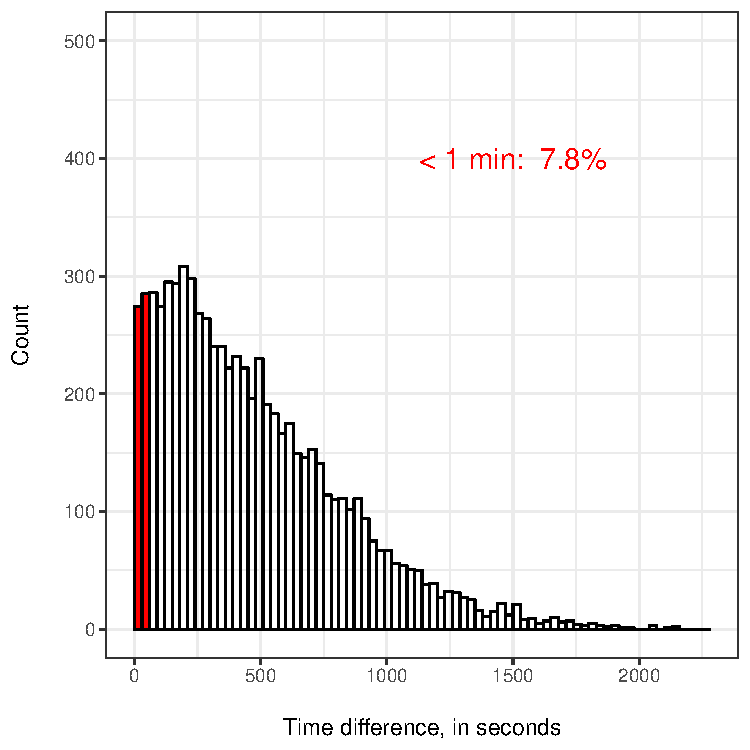
\includegraphics[width=\textwidth,
    keepaspectratio]{simulated_time_with_age.pdf}
    \caption{Differences in Hahner finishing times}
    \label{fig:simulatedfinishtimes}
  \end{subfigure}
  \begin{subfigure}{.45\textwidth}
    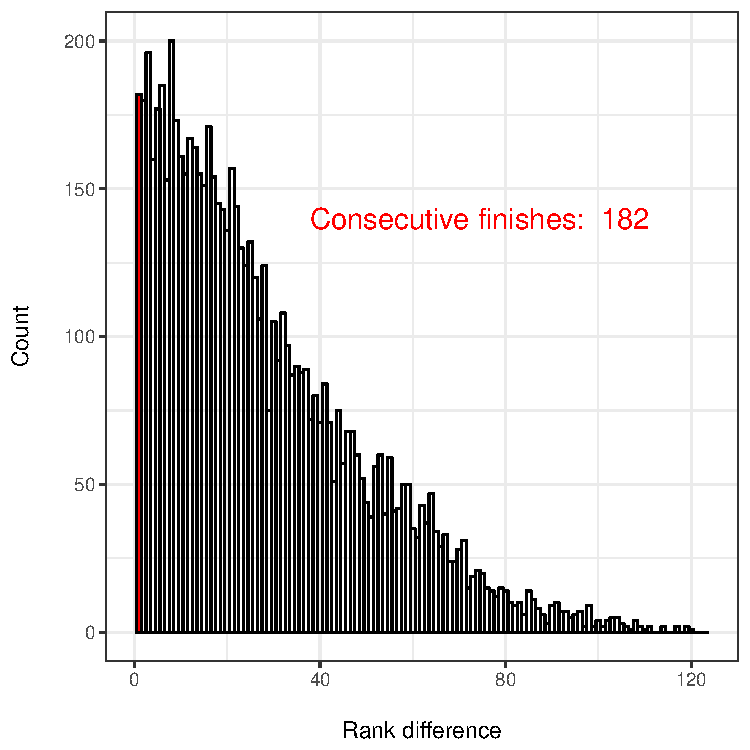
\includegraphics[width=\textwidth, keepaspectratio]{simulated_rank_with_age.pdf}
    \caption{Differences in Hahner twin places}
    \label{fig:simulatedranks}
  \end{subfigure}
\end{figure}

The histograms in Figure \ref{fig:simdiff} raise questions about the
credibility of Anna and Lisa Hahner's story and in particular suggest
that a simultaneous finish in the Rio marathon would be very rare if
Anna and Lisa had run independently. For example, in fewer than 300 of
10,000 simulated races did Anna and Lisa Hahner finish within 30
seconds of one another, and in fewer than 600 did the Hahner twins
finish within a minute of each other.  The histogram area associated
with this latter result is depicted in red in Figure
\ref{fig:simulatedfinishtimes}.  Moreover, the Hahner twins finished
in consecutive rank in fewer than 200 of 10,000 simulated races; the
red zone in Figure \ref{fig:simulatedranks} presents this visually.
The close finish that was observed in Rio, where Anna and Lisa crossed
the finish line one after the other, would have been highly unlikely
if the two German twins had raced independently of each other.

Parallel with our prior analyses, we repeated our simulations using
half marathon splits as the predicting variable in our simulations;
results are in Figure \ref{fig:simdiffhalf}.  While this use of
marathon splits reduces the variation in the predicted outcome of each
runner and therefore reduces the expected distance between Anna and
Lisa Hahner, even with half marathon split as a measure of ability it
is still quite rare for the twins to finish simultaneously or
consecutively.

\begin{figure}[!ht]
  \centering
  \caption{Distribution of Hahner twin results in 10,000 simulated
    marathons, based on half marathon splits}
  \label{fig:simdiffhalf} 
  \begin{subfigure}{.45\textwidth}
    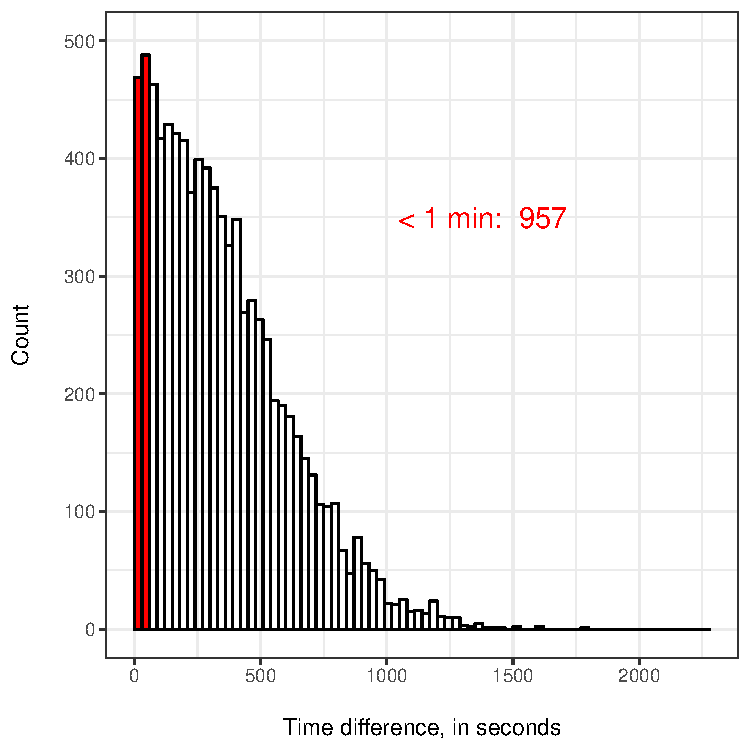
\includegraphics[width=\textwidth,
    keepaspectratio]{simulated_time_half_with_age.pdf}
    \caption{Simulated differences in finishing times}
    \label{fig:simulatedfinishtimes_half}
  \end{subfigure}
  \begin{subfigure}{.45\textwidth}
    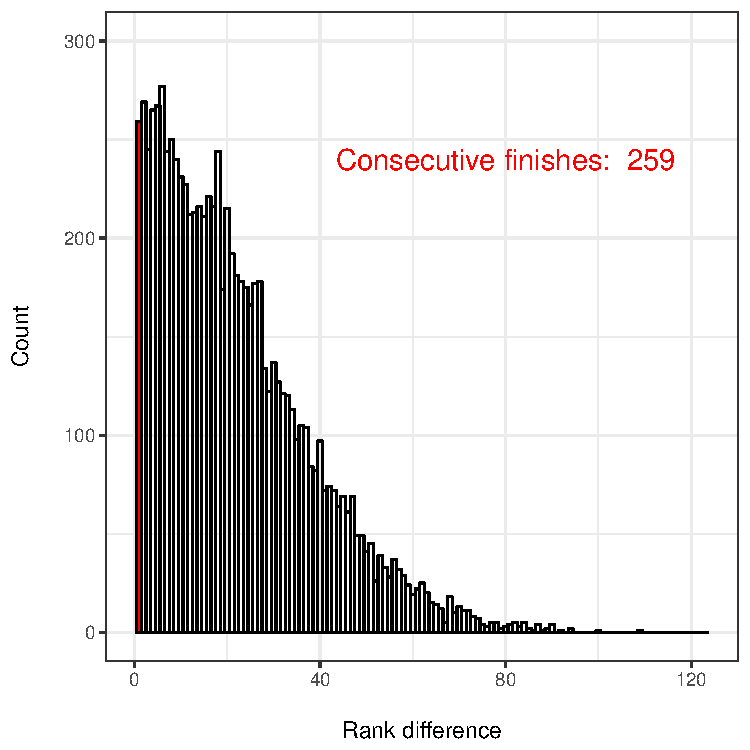
\includegraphics[width=\textwidth, keepaspectratio]{simulated_rank_half_with_age.pdf}
    \caption{Simulated differences in places}
    \label{fig:simulatedranks_half}
  \end{subfigure}
\end{figure}

The way that we handled DNFs in our simulations is notable. As our
description above indicates, we assumed that DNF probabilities are the
same for all runners and that the likelihood of a DNF is not a
function of a runner's anticipated marathon finishing time. The rug
marks in Figure \ref{fig:45degreeplot} suggest that runners with
better personal best times may be more likely to DNF than other
runners, all things equal. We suspect that this occurs because some
better runners may expend excessive energy trying to achieve a good
result in the marathon and in so doing injure or exhaust themselves;
lesser runners, in contrast, may be content to finish
respectably. Regardless of the validity of this conjecture, Figure
\ref{fig:45degreeplot} shows that the Hahner twins are representative
of the sort of runners who DNFed in Rio. Since our simulated Hahner
statistics are conditioned on both Hahner twins finishing, it follows
that they are conservative. The fact that both women finished the
marathon was notable in and of itself, and by discounting the
possibility of a Hahner DNF we are giving the benefit of the doubt to
the Hahner twins.

\section*{Conclusion}

We have studied Anna and Lisa Hahner's near-simultaneous finish in the
2016 women's Olympic marathon in Rio. This finish elicited a
controversy insofar as the German twins were accused of deliberately
slowing down and finishing next to each other so as to generate media
attention. They denied this, not entirely surprisingly,

We have offered two perspectives on the marathon, one based on
visualizations and simple calculations and a second that draws on a
simulation. Both perspectives have the same implications, and they are
as follows. In a global sense, the Hahner twins did not slow down
appreciably during the Rio marathon. Their times were not fast, but
they were within reason for runners of the Hahners' abilities and age.
Locally, though, we find that the Hahners' finish was in fact probably
contrived. Their finish---consecutive, with one second between the two
women---was a rather low probability event. Compared to their
differences in talent, that is, the Hahner twins difference in
finishing times was unusually compressed. This is evidence that their
finishing had elements of intentionality---perhaps at the last minute
but intentionality nonetheless.

Our goal is not to speak to the question of whether the Hahner twins
should or should not have enjoyed what some might call an artificial
moment of Olympic glory. Neither was in contention for a podium finish
in Rio, and compared to the doping allegations that presently surround
endurance sports in general, what the Hahners appear to have done
seems relatively tame. Still, it might have behooved them to have been
a bit more open about their end-of-race tactics, and to this end we
have shown here how a simple data analysis can shed light on claims
about racing results.  Should the 2020 Summer Olympics again feature
marathoning twins and triplets, we look forward to a comparative
analysis using the techniques illustrated here.





\section*{Further reading}

\begin{itemize}

\item \url{http://www.telegraph.co.uk/olympics/2016/08/17/german-twins-criticised-for-finishing-olympic-marathon-fun-run-h}

\item
  \url{https://www.nytimes.com/2016/08/17/sports/olympics/twins-finish-marathon-hand-in-hand-but-their-country-says-they-crossed-a-line.html}

\item
  \url{https://www.welt.de/sport/olympia/article157669264/Das-falsche-Laecheln-der-deutschen-Lauf-Zwillinge.html}
\end{itemize}

\end{document}

